\subsection{Digital Signals}

\begin{figure}[h!]
    \centering
    \includegraphics[width=\textwidth]{img/digital\_analog\_signal.png}
    \caption{Analog vs Digital Signal}
    \label{fig:analog_digital}
\end{figure}

\subsubsection{Continuous-time sinusoidal signal}
Continuous-time sinusoidal signal is formally written as
$$
x(t)=A \cos (\Omega t+\theta)=A \cos (2 \pi F t+\theta), t \in \mathbb{R}
$$

\begin{itemize}
    \item $A$ is amplitude
    \item $\Omega$ is the angular frequency (radians/second)
    \item $F$ is the frequency $\left(\mathrm{s}^{-1}=\mathrm{Hz}\right)$
    \item $T_p=F^{-1}$ is the period (s)
    \item $\theta$ is phase (radians)
\end{itemize}
\noindent
Complex signal continuous-time sinusoidal signal
$$
x(t)=e^{j(2 \pi F t+\theta)}=\cos (2 \pi F t+\theta)+j \sin (2 \pi F t+\theta)
$$
Complex representation of real sinusoidal
$$
A \cos (2 \pi F t+\theta)=\frac{A}{2} e^{j(2 \pi F t+\theta)}+\frac{A}{2} e^{-j(2 \pi F t+\theta)}
$$

\begin{figure}[h!]
    \centering
    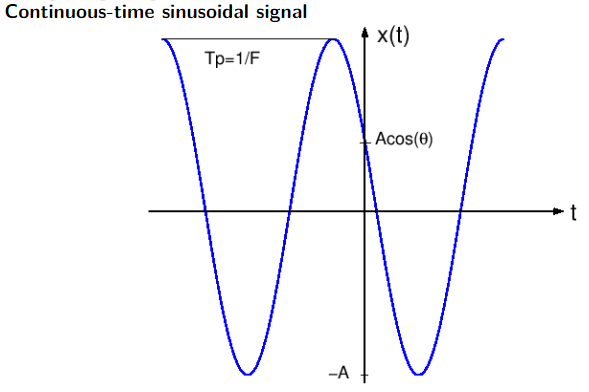
\includegraphics[width=\textwidth]{img/sinusoidal.PNG}
    \caption{Continuous-time Sinusoidal}
    \label{fig:sinusoidal}
\end{figure}

\subsubsection{Fourier transform}
Decomposition into complex harmonics
If $x(t)$ is periodic with period $T_p=1 / F_0$ then
$$
x(t)=\sum_{k=-\infty}^{\infty} c_k e^{j 2 \pi k F_0 t}
$$
- $x(t)$ is constructed from the set of basis signals:
$$
\left\{k \in \mathbb{Z}: e^{j 2 \pi k F_0 t}\right\}
$$
- The complex Fourier coefficients $c_k$ determine the shape of the period signal

\clearpage
\textbf{Example}
\begin{figure}[h!]
    \centering
    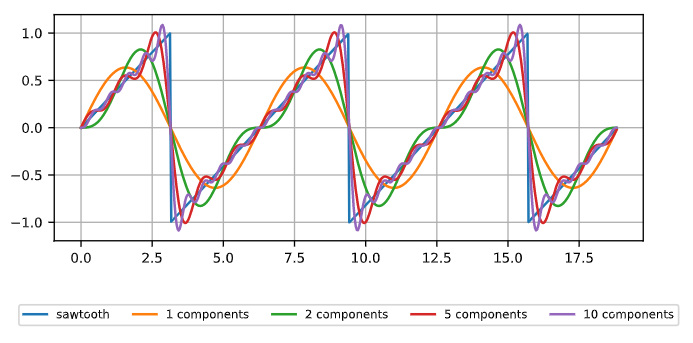
\includegraphics[width=\textwidth]{img/fourier.PNG}
    \caption{Example Fourier Decomposition of Signal}
    \label{fig:fourier}
\end{figure}
\noindent
\begin{center}
Analysis: $\quad c_k=\frac{1}{T_p} \int_{T_p} x(t) e^{-j 2 \pi k F_0 t} d t$

Synthesis: $\quad x(t)=\sum_{k=-\infty}^{\infty} c_k e^{j 2 \pi k F_0 t}$
\end{center}
The periodic signal onto its Fourier spectrum (coefficients) is a bijective mapping. Bijective
means that there is a “one–to–one” correspondence.